\chapter{評価}
\label{chapter:evaluation}

本章では, $\S$\ref{chapter:proposal}にて提案した, データセンターレーンモデルにおける経路切り替え手法の性能評価を示す. 
性能評価については, 3つのパートに分かれている. 
一つ目は, 提案手法の基本的な性能について, 提案手法が設定するパラメータによってどのような挙動を示すのかを評価する. 
二つ目は, $\S$\ref{chapter:proposal}にて示したデータセンタートラフィックがもたらす性能障害に対して,
提案手法を用いた結果どのように改善されたのかを評価する. 
そして最後に, データセンターネットワークが生成するトラフィックに対する評価として, トポロジー,
トラフィック分布の点で実際のデータセンター環境に近いものを想定し, 性能評価を行う. 

\section{実験環境}
この章での評価実験は全てシミュレーション上で行ったものである.
シミュレーションには, パケットレベルでのシミュレーションが可能なns-3 DCE(Direct Code
Execution)\cite{ns3}を用い, Linuxカーネルに実装した提案手法を用いて評価実験を行った.
それぞれの評価実験において, エンドノードにおける輻輳制御にはTCP New Renoを用いた. 
一般的に, データセンタースイッチは各ポート$128-256KB$バッファが割り当てられている\cite{dctcp}. 
今回の実験ではこの制約に従い, キュー長は$128KB$の入出力バッファを用意している. 
また, 各スイッチのレイテンシとして, $25 \mu s$に設定した. 
この遅延時間も一般的なデータセンターの値となっており\cite{dctcp}, 以下のような各遅延の影響に関する考察においても,
妥当であることがわかる\cite{detail}

\begin{itemize}
\item 伝送遅延 $12.24\mu s$ : 1Gbpsリンク1530バイトイーサネットフレームの遅延量. 
\item クロスバー遅延 $3.06\mu s$ : クロスバーspeedup-factor=4における遅延量.
HOLブロッキングを抑えるために一般的にこの値が設定されている\cite{crossbar}. 
\item 伝搬遅延 $0.476\mu s$ : 銅線における遅延量\cite{delay}.
\item 送受信処理遅延 $5\mu s$\cite{delay}
\item フォワーディング遅延 $4.224\mu s$フォワーディングエンジンによる遅延量($25\mu s$の残り分)
\end{itemize} 

% \subsection{トポロジー}
% 今回の評価実験では, Multi-homing FatTreeトポロジー(k=4)を用いて評価を行った\cite{fattree}. 
% 4-pod MHFTトポロジーでは, 異なるポッドでのノード間通信において, 2つの等コストな経路がある. 
% ノードの数だけある各エッジスイッチに対し, 2つのノードが接続する. 
% このトポロジーでは16台のノードと2台のコアスイッチがある. 
% それぞれのスイッチは4-port 100Mbpsスイッチで, 通信容量についてボトルネックはない. 

\subsection{評価メトリック}
既存の取り組み\cite{dctcp, d3, pdq}のように, 二つのメトリックを用いて評価を行う. 
通信時間にデッドラインが設けられているような, レイテンシ指向のフローについては, FCTを用いる. 
FCTについても, 平均値だけでなく, テール部分に着目した95パーセンタイルFCTを導入する. 
テール部分で見られる大きな遅延については, OLDIアプリケーションのような, 各クエリーに対して最も遅いレスポンスを待ち,
最終的な処理時間となるようなタスクでの重要な指標となる\cite{survey}. 
より多くのデータを通信したいスループット指向のトラフィックについては, 各フロー毎のスループットを用いる. 


\subsection{比較対象}
今回の評価実験では, Pure-MPTCP\cite{mptcp}とRepFlow\cite{repflow}についても評価実験を行い,
提案手法との比較を行った.
比較する手法について以下にまとめる.

{\bf Pure-MPTCP}\cite{mptcp}: 提案手法の評価におけるベースラインとしてMPTCP-New Renoを用いる. 
$Initial window$として12パケットに設定している. 
また, スイッチの入出力キューはDropTailに従うように設定している. 
その他の設定は, 既存の取り組みを参考にした\cite{d2tcp, p_fab}.
今回の評価では, MPTCPのソースコードとしてMPTCP v0.88を用いる. 
また, 今のMPTCP実装では約80KB以下のフローに対しては複数の経路を用いず, Singlepath-TCPと同様の挙動となる. 

{\bf RepFlow}\cite{repflow}: エンドーノードへのアプローチに焦点を当てた,
最先端のショートフロー短縮化技術としてRepFlowを用いる. 
RepFlowはスイッチ, エンドノードのカーネルへの変更が不要な手法であり, 複数の経路を持つ今日のデータセンターネットワークに対して,
輻輳の起こっている経路を回避するため, 通信可能で等コストな経路にショートフロー通信を複製する. 
これにより, キューイング遅延の影響を確率的に減らすことができ, 結果的に最短時間で到着したフローによって短縮化することができる.
今回の評価では, 100KB以下の全てのフローに対して複製を行う\cite{repflow}. 
その他のパラメータはPure-MPTCPと同じである. 

{\bf デッドラインベースの経路切替手法}: 

$\S$\ref{chapter:proposal}にて示した,
デッドライン時間に基づいた単純な切り替え手法である.
切り替えのタイミングにはパラメータ$t_{deadline}$を用いる. 
評価実験では, $t_{deadline}=300[ms]$と設定する.

{\bf リンクコストベースの経路切替手法}: 

$\S$\ref{chapter:proposal}にて示した各経路状況に対応した経路切り替え手法である. 
切り替えのタイミングにはリンクコストを用いる. 
基本的に評価実験では, $t_{deadline}=300[ms]$, $\alpha=1, \beta=1, \gamma=1,
\delta=1$と設定する.

\section{基本性能:スループット}
初めに, 提案手法の基本的な性能として, 従来手法と提案手法の挙動の違いとして, 時系列でのスループットの変化について示す.  
提案した二つの手法には, 予め設定するパラメータとして$t_{deadline}, \alpha \sim \delta$があるが, $\alpha
\sim \delta$については固定し, $t_{deadline}$を変化させることで経路切替による通信性能の影響について評価する. 
この評価ではエンドノード間の1対1の通信を想定しており, ベンチマークトラフィックには,
iperfを用いて2秒間継続してデータ転送を行った. 
またトポロジーとしては, Fig.\ref{fig:lane_model}のようなエンドノード間の等価な通信経路が3つあり, そのうち1つをSL,
残りの2経路をLLに割り当てているものを用いる.
すなわち, 提案手法の制御において通信開始時には, SLの最大1経路分とLLのウィンドウサイズ1分ののスループットが可能であり, 経路切替が生じた後,
最大2経路分のスループットを出すことができる.
なお, Pure-MPTCPでは現状の実装上最大2経路分, RepFlowでは基本的にTCPでの適用を想定しているため,
最大1経路分のスループットを達成することが可能である. 

Fig.\ref{fig:basic_comparison}に上記の評価結果として, 時系列ごとのスループットの変化を示す. 
この結果から, 提案手法の経路切替の際にデータ転送量の増加率に劣化が見られるものの, 約100[ms]以内には元の増加率に戻ることがわかる. 
これは, 提案手法では, 経路が切り替わる前の時点ではSLはウィンドウサイズ1に設定しているため,
経路切替が発生した直後のウィンドウサイズ増加アルゴリズムとして, スロースタートの挙動を示す. 
そのため, スループット増加の傾きが緩やかになる. 
また, 200ms付近での増加しきった後, 性能劣化する挙動については輻輳制御が働いていることと,
サブフローでの通信においては従来の輻輳制御を無視し, 強制的に1に設定するため, 急激にスループットが下がり, 一経路分の通信性能へと落ち着く. 
また, デッドラインベースの切替手法では300ms時に切替が生じたが, リンクコストベースの切替手法では約180ms時に切替が生じた. 
これは, リンクコスト算出の際のキューイング遅延の項の影響を受け, より早く経路が切り替わるという判断がされたためである. 
% 
% \begin{figure}[t]
%     \begin{center}
%     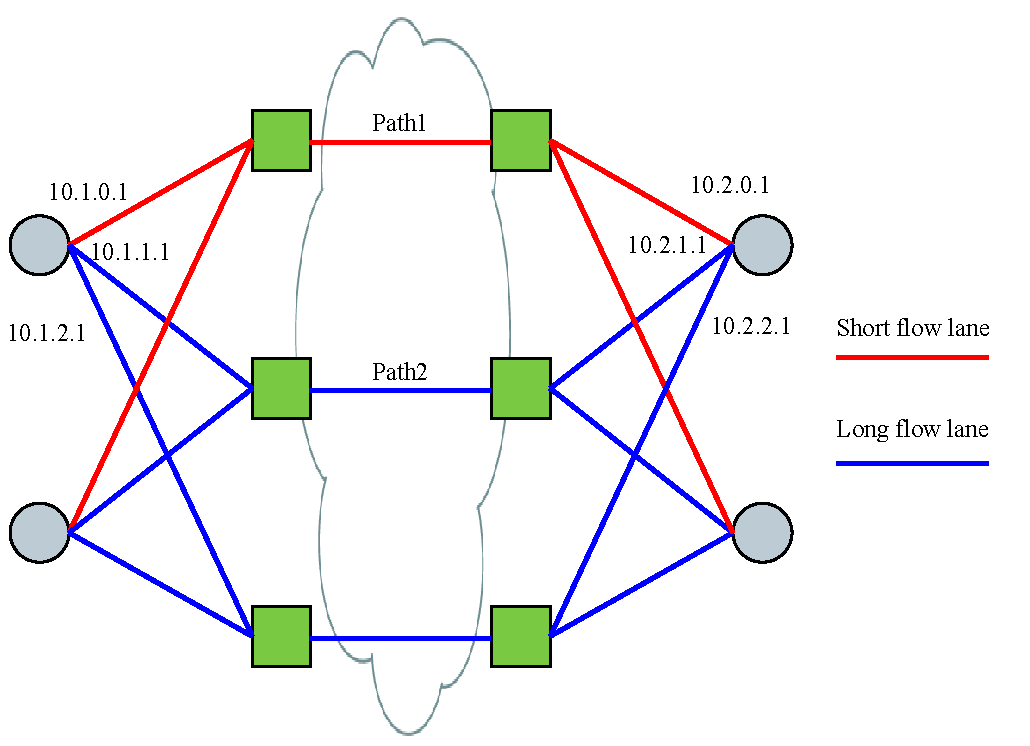
\includegraphics[autoebb, width=250pt]{./img/lane_model.pdf}
%     \caption{Datacenter Lane Network Model}
%     %\ecaption{The control loop in DCTCP}
%     \label{fig:lane_model}
%     \end{center}
% \end{figure}


\begin{figure}[t]
    \begin{center}
    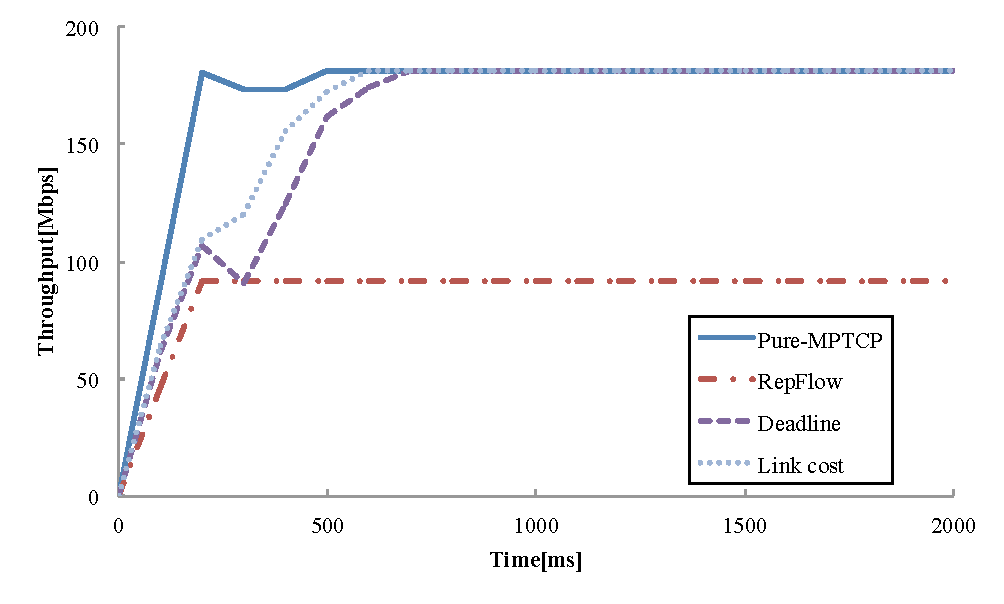
\includegraphics[autoebb, width=250pt]{./img/basic_comp.pdf}
    \caption{Basic performance comparisons}
    %\ecaption{The control loop in DCTCP}
    \label{fig:basic_comparison}
    \end{center}
\end{figure}

次に,
デッドラインベースの切替手法について$t_{deadline}$を$30,
300, 1000$へ変化させた時の時系列でのスループットの変化の違いをFig.\ref{fig:basic_deadline}に示す.
この結果から, $t_{deadline}$を変化させることで, パラメータに応じた切替が達成できていることがわかる. 
それぞれの挙動については先に述べたように, スロースタートによる輻輳制御と強制的にウィンドウサイズを1に設定した時の挙動を示している. 

\begin{figure}[t]
    \begin{center}
    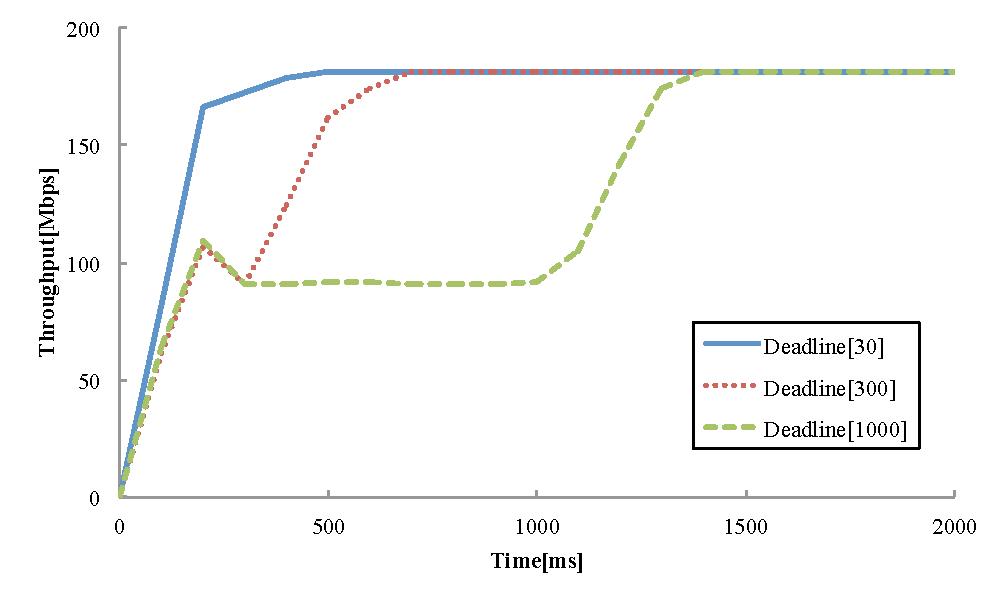
\includegraphics[autoebb, width=250pt]{./img/basic_dead.pdf}
    \caption{Basic performance path switching based on deadline}
    %\ecaption{The control loop in DCTCP}
    \label{fig:basic_deadline}
    \end{center}
\end{figure}


次に,
リンクコストベースの切替手法について$t_{deadline}$を$30,
300, 1000$へ変化させた時の時系列でのスループットの変化の違いをFig.\ref{fig:basic_cost}に示す.
この結果から, $t_{deadline}$を変化させることで, パラメータに応じた切替が達成できていることがわかる. 
また, この手法では$t_{deadline}$は主要なパラメータの一つではあるが, 式\ref{linkcost}が示すように,
他のリンクの状況に対応して経路切替時間はが変化する. 


\begin{figure}[t]
    \begin{center}
    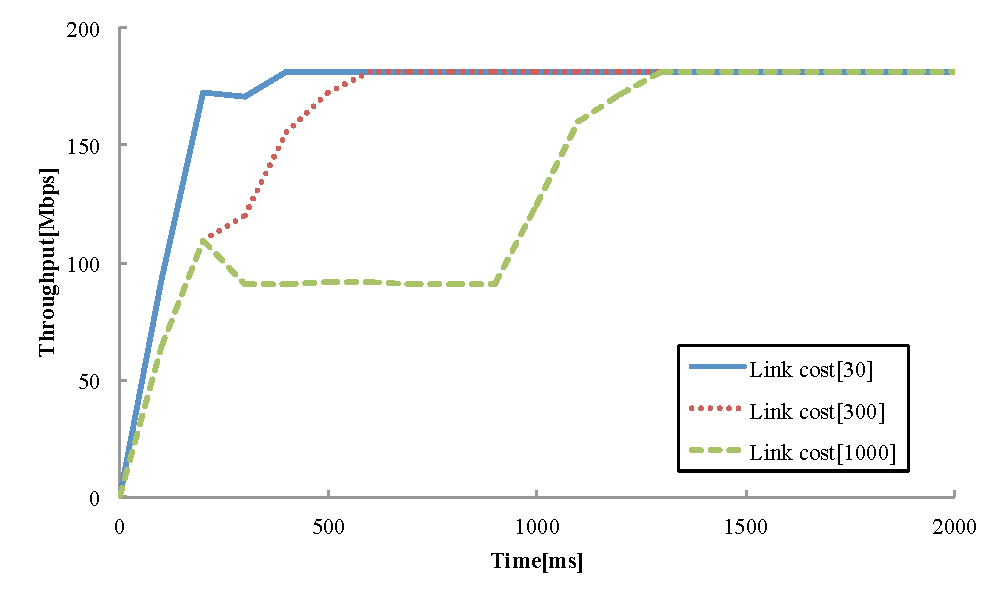
\includegraphics[autoebb, width=250pt]{./img/basic_cost.pdf}
    \caption{Basic performance path switching based on
    link-cost}
    %\ecaption{The control loop in DCTCP}
    \label{fig:basic_cost}
    \end{center}
\end{figure}

\section{基本性能:切替時間}
次にリンクコストベースの切替手法における各パラメータ毎の挙動の違いを示す. 
デッドラインベースの切替手法とは異なり, リンクコストベースの切替手法では各リンクの経路状況を表すためのリンクコスト値があり, パラメータ$\alpha \sim
\delta$がある. 
各パラメータの意味についてはTable.\ref{table:link_cost_nature}の通りであり,
これらを変化させることで, 各リンクの通信状況に対する経路切替の挙動の変化を通信開始から経路切替が発生するまでの時間によって示す.
この評価ではエンドノード間の1対1の通信を想定しており, ベンチマークトラフィックには,
iperfを用いて継続してデータ転送を行った.  
また, トポロジーとしてk=4 MHFTを用いる. 
このトポロジーでは, エンドノード間の等価な通信経路が2つあり, それぞれSLとLLに割り当てている. 
それぞれのレーンに対し通信負荷を与えることで経路の状況を変化させる. 
SLに対する通信負荷には, 64KBのフローを200msに1回ポアソン生起するトラフィックを用いる. 
LLに対する通信負荷には, 実験時間中継続してデータ転送を行うトラフィックを用いる. 
それぞれの通信負荷については, Senderノードの数を変化させ, 負荷の度合いに対する評価を行う. 
なお, パラメータ$t_{deadline}$は$300[ms]$を設定している. 

経路状況に対する挙動に関わるパラメータ$\alpha,
\beta$を変化させたときの経路切替時間の移り変わりをFig.\ref{fig:basic_para_link}に示し, 横軸はSL,
LLへの通信負荷の強度を表すSenderノードの数, 縦軸には通信が発生したときの時間を0としたときの経路切替時間を示している. 
この結果から, パラメータ$\alpha$が大きくなればなるほど, 経路状況の変化にアグレッシブに反応し, また値が小さいと
パラメータ$t_{deadline}$の影響を大きく受けることとなり, 設計目的の期待の狙い通りの結果が得られた. 
実際, SLでのSenderノードが増えれば増えるほど, SLでのキューイング遅延が大きくなり, SLのリンクコストの値が大きくなる. 
これは, SLで通信をするよりもLLで通信を行ったほうが有利であると判断された結果であり, このため切替時間が短くなる. 
また, LLでのSenderノードが増えれば増えるほど, LLでのキューイング遅延が大きくなり, LLのリンクコストが大きくなる. 
これは, LLへ切り替えて通信するよりもSLに留まって通信を継続した方が有利であると判断された結果であり, このため切替時間が長くなる. 

\begin{figure}[t]
    \begin{center}
    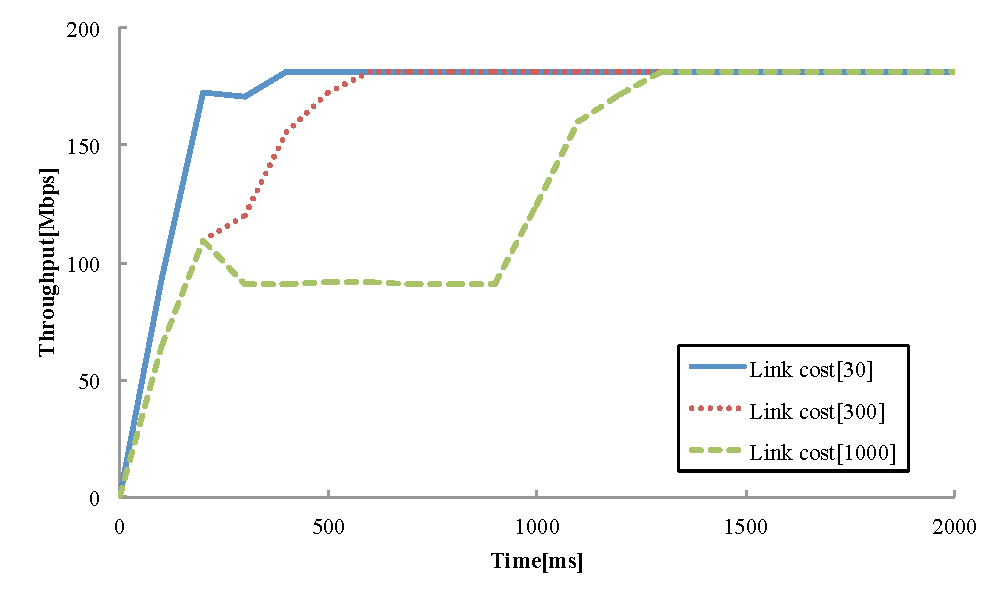
\includegraphics[autoebb, width=300pt]{./img/basic_cost.pdf}
    \caption{Basic performance path switching based on
    link-cost}
    %\ecaption{The control loop in DCTCP}
    \label{fig:basic_para_link}
    \end{center}
\end{figure}


次にデッドラインに対する挙動に関わるパラメータ$\gamma,
\delta$を変化させたときの経路切替時間の移り変わりをFig.\ref{fig:basic_para_dead}に示す.
この結果から, パラメータ$\gamma$が大きくなればなるほど, 経路状況よりも$t_{deadline}$に大きく依存することとなり,
設計の狙い通りの結果が得られた.
実際, LLでのSenderノードが増えれば増えるほど, LLでのキューイング遅延が大きくなり, SLに留まるような判断がされるが,
$t_{deadline}$を超えれば経路切替が発生しやすくなるような挙動をする.
そのため, 切替時間が$t_{deadline}$を大きく超えるような挙動は発生しない. 

\begin{figure}[t]
    \begin{center}
    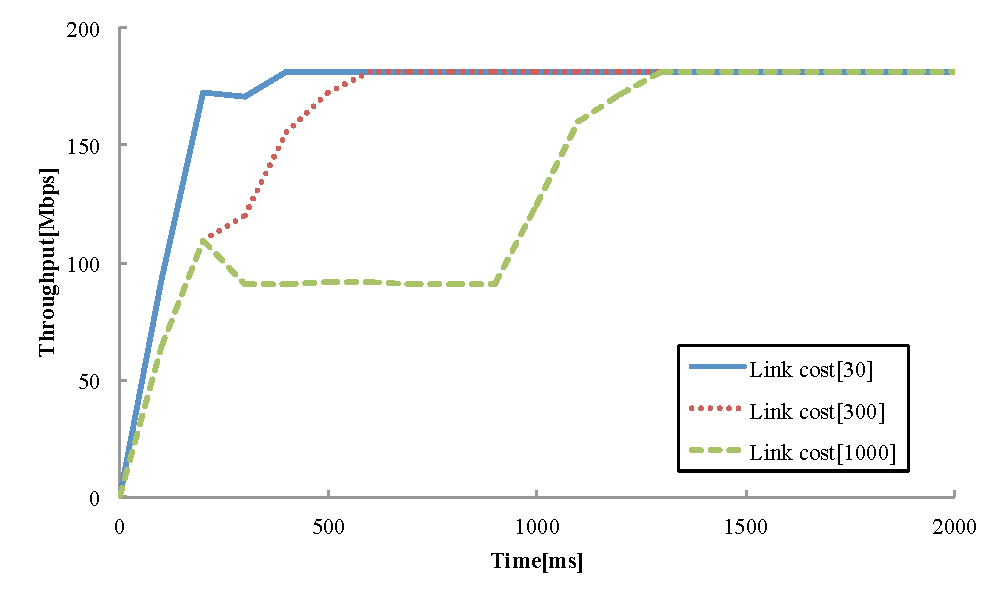
\includegraphics[autoebb, width=300pt]{./img/basic_cost.pdf}
    \caption{Basic performance path switching based on
    link-cost}
    %\ecaption{The control loop in DCTCP}
    \label{fig:basic_para_dead}
    \end{center}
\end{figure}

\section{性能障害:Queue buildupに対する性能評価}
次に$\S$\ref{sec:expected_effect}にて示した, Queue buildupに対する評価を行う. 
Queue buildupではスイッチの一つのインタフェースに継続的にデータ転送を起こすロングフローとショートフローが混在し, ロングフローがキューを占有し,
その結果, サイズの小さいショートフローが遅延する. 
この性能障害に対する提案手法の評価としてFig.\ref{fig:eval2_topo}に示す, k=4 DHFTベースのトポロジーを用いる. 
このトポロジーでは, エンドノード間の2つの等価な通信経路にそれぞれSLとLLに割り当てている.
また8台のエンドノードに対して, 25\%のノード(2)をバックエンドノード, 75\%のノード(6)をフロントエンドノードと想定する. 
ベンチマークトラフィックには, バックエンドノードに対し, 実験時間中継続してデータ転送を行うトラフィックを用いる.
また, 全てのバックエンドノードへの通信負荷を与えることで, Queue buildupの影響の大きさを変化させる. 
通信負荷については, Senderノードの数を変化させ, 負荷の度合いに対するショートフロー性能の評価を行う. 
さらに, 全てのフロントエンドノードに対し, ロングフロー通信開始よりも前の時間から$64KB$のショートフローを200msに1回ポアソン生起させる. 
これにより, 二種類のトラフィックが同時に開始することとなる. 
この時のショートフローのFCTを評価することで, 提案手法のQueue buildupに対する改善を評価する. 
評価の際のメトリックとしてはショートフローの平均FCTと, 95パーセンタイル値を用いる. 
特に遅延した下位5パーセントに着目することで, 遅延した割合の大きさを比較することができ, 
本研究の目的である, コンスタントにアプリケーション性能の出せるデータセンターネットワークの実現への指針となる.
このシミュレーションでは, ポアソン生起を用いたショートフローの発生間隔についてランダム性が発生し, 100回シミュレーションを繰り返し行った. 
また, 提案手法のパラメータには, $t_{deadline}=300[ms]$, $\alpha=1, \beta=1, \gamma=1, \delta=1$と設定する.

\begin{figure}[t]
    \begin{center}
    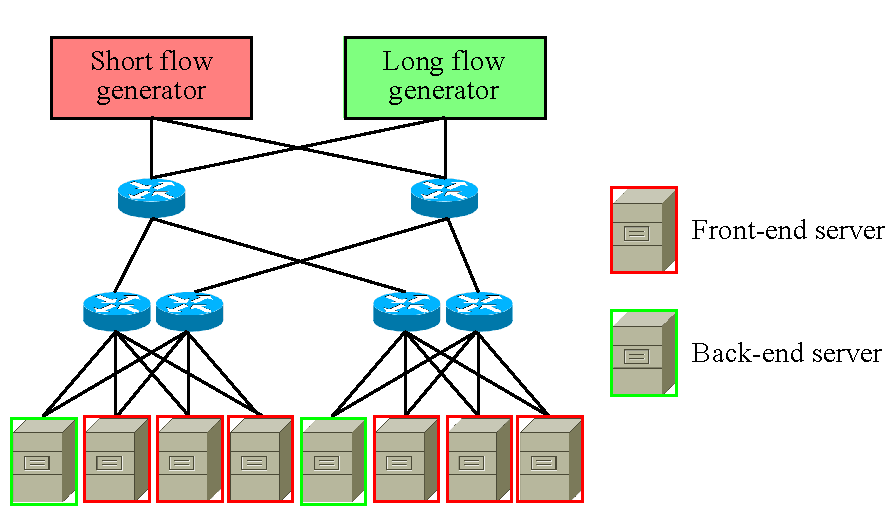
\includegraphics[autoebb, width=300pt]{./img/evalu2.pdf}
    \caption{Topolgy for impairment of Queue buildup evaluation}
    %\ecaption{The control loop in DCTCP}
    \label{fig:eval2_topo}
    \end{center}
\end{figure}

Fig.\ref{fig:eval2_aver}にQueue buildupでの64KBショートフローの平均FCTを示す. 
横軸は, バックエンドノードに対する通信負荷の度合いを示すSenderノードの数, 縦軸には平均FCTを示す. 
この結果から, 提案手法ではショートフローに対するロングフロー通信負荷の影響を軽減させていることがわかる. 
これはレーンモデルと経路切替手法によって, バックエンドに対するロングフローはLLへと切り替えられ,
フロントエンドに対するショートフローは良好な経路状況であるSLで通信することができるため, FCTが短縮化することができていることが理由である. 
一方,  Pure-MPTCPではSenderノードが1台の時でも, 2経路を同時に利用しながら通信するため,
通信負荷が小さい段階から大きく遅延していることがわかる. 
また, RepFlowではロングフローは1経路分しか利用しないため, 通信負荷が小さい段階では, 輻輳の影響が小さく, 平均FCTも小さいが,
通信負荷を大きくしていくと, 2経路に対する利用率が大きくなり, FCTが遅延する. 

\begin{figure}[t]
    \begin{center}
    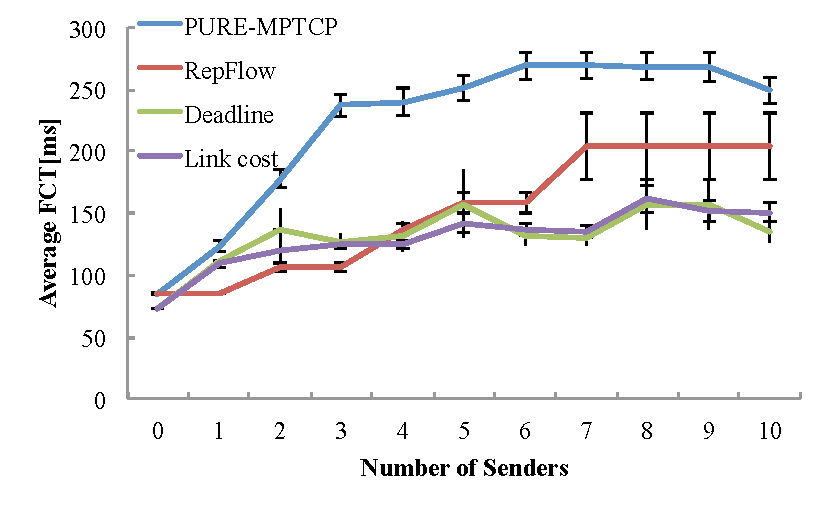
\includegraphics[autoebb, width=300pt]{./img/eval2_avr.pdf}
    \caption{Short flows average FCT in Queue buidup}
    %\ecaption{The control loop in DCTCP}
    \label{fig:eval2_aver}
    \end{center}
\end{figure}

次に, Fig.\ref{fig:eval2_tail}にQueue buildupでの64KBショートフローの95パーセンタイルFCTを示す. 
横軸は, バックエンドノードに対する通信負荷の度合いを示すSenderノードの数, 縦軸には95パーセンタイルFCTを示している. 
この結果から, 二つの提案手法では, 大きな遅延が生じたフローの割合についても改善できていることがわかり, 特にリンクコストベースの切替手法では,
デッドラインベースのものと比べ, より大きく改善できている. 
提案手法において, 特に遅延が生じるのはロングフローが発生した直後のSLを用いて通信を行う時間に,
ショートフローが発生した場合である.
デッドラインベースの経路切替手法で経路の状況によらず, $t_{deadline}$時間中は必ずSLにて通信が行われ, その際にショートフローが遅延する. 
これに対し, リンクコストベースの経路切替手法では, 経路状況に合わせて切替時間が変化するため,
SLで通信を行っているレイテンシ指向なフローに対する影響を抑制することで, FCT改善の改善を達成した. 
一方で, RepFlowについては, 通信負荷が小さい時には遅延しているフローの割合は小さい. 
これは, 提案されたRepFlowではTCP通信を想定しているため, バックエンドノードに対するトラフィックも1経路分の負荷しかかけることができない. 
そのため, 他のMPTCPによる手法と比較して約半分の通信負荷となっており, 通信負荷が小さい時にはRepFlowによるフローの複製が有効に機能する. 
しかし, 通信負荷が大きくなるとキューイング遅延が大きい経路を選択せざるを得なくなるため, 遅延が生じる. 
そのような状況においても, RepFlowによる手法ではPure-MPTCPよりは改善が見られる. 

今回の評価実験では, ショートフローが通信している中でロングフローが通信開始するため,
SLの経路状況はLLよりも悪化していると考えられる.
そのためリンクコストベースの経路切替手法の挙動として, 切替時間がデッドライン時間よりも短くなり, LLへ切り替わる時間が早くなる. 
その結果, SLにてショートフローとロングフローが混在する時間が短くなり, 遅延したフローの割合が小さくなる. 
一方で, 二種類のフローを分類して通信する提案手法,
特に経路状況に対応して通信することができるリンクコストベースの経路切替手法では大きく改善できたのに対し, Pure-MPTCPとRepFlowについては,
それぞれ二種類のトラフィックを混在させ通信を行うため, 遅延する割合が大きくなり, ショートフロー通信の性能が劣化する. 


\begin{figure}[t]
    \begin{center}
    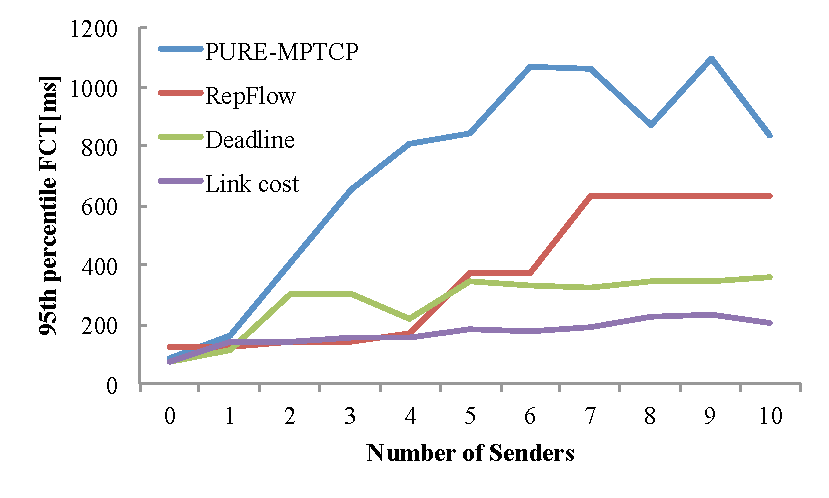
\includegraphics[autoebb, width=250pt]{./img/eval2_tail.pdf}
    \caption{Short flows $95^{th}$ FCT in Queue buidup}
    %\ecaption{The control loop in DCTCP}
    \label{fig:eval2_tail}
    \end{center}
\end{figure}


\section{実環境でのトラフィックを想定した性能評価}
最後に, 実際のデータセンター環境を想定した評価実験を行った. 
この評価ではトポロジーとして, k=4 DHFTを用いる. 
このトポロジーでは, エンドノード間の2つの等価な通信経路にそれぞれSLとLLに割り当てている.
また16台のエンドノードに対して, 先ほどの評価実験と同様に25\%のノード(4)をバックエンドノード,
75\%のノード(12)をフロントエンドノードから構成されている環境を考える. 

ベンチマークトラフィックとしては, 二つのデータセンターアプリケーションを想定する. 
一つは, ウェブ検索を想定したトラフィック\cite{dctcp}である. 
このトラフィックでは, 全体の95\%以上のトラフィック量が, 全体割合の内30\%以下である1MB以上のデータによってもたらされているとい
う特徴がある. 
もう一方は, データマイニングトラフィックである\cite{vl2}. 
このトラフィックでは, 全体の95\%以上のトラフィック量が, 3.6\%以下の割合であ35MB以上のデータによってもたらされており, 一方で,
80\%以上の割合が, 10KB以下のフローである. 
これら二つのトラフィックは大きなテール状の分布をしており, ショートフローとロングフローが混在している. 
今回の評価実験では, これらのトラフィックに対しテール状の確率分布を表現できるパレート分布を用いて生成した.  
Fig.\ref{fig:websearch}, \ref{fig:datamining}にそれぞれのトラフィックの分布を示す. 
また, Table.\ref{table:workload}にそれぞれのトラフィックを生成するための統計情報を示す. 
さらに, バックエンドノードに対するトラフィックによる通信負荷を変化させた時の評価を行う. 
具体的には, バックエンド, フロントエンドそれぞれに対し, 通信対象となるノードの割合を$Load$とし, これを$Load=0.1 \sim
0.8$まで変化させる. 

\begin{figure}[t]
    \begin{center}
    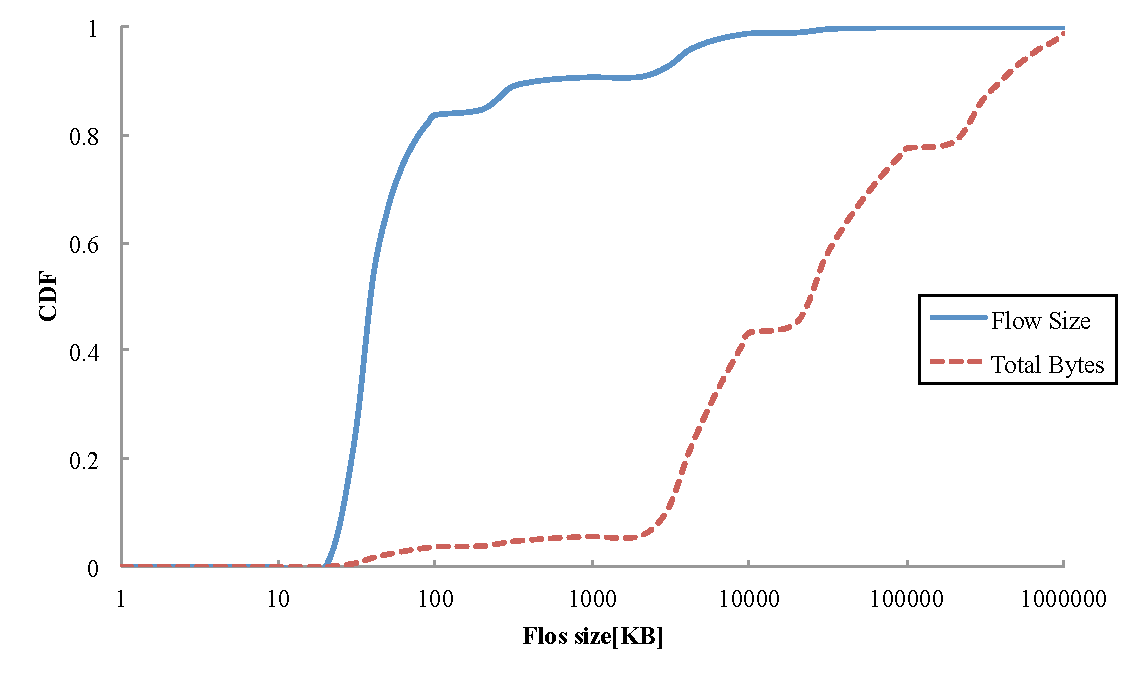
\includegraphics[autoebb, width=250pt]{./img/websearch.pdf}
    \caption{Web search workload}
    %\ecaption{The control loop in DCTCP}
    \label{fig:websearch}
    \end{center}
\end{figure}

\begin{figure}[t]
    \begin{center}
    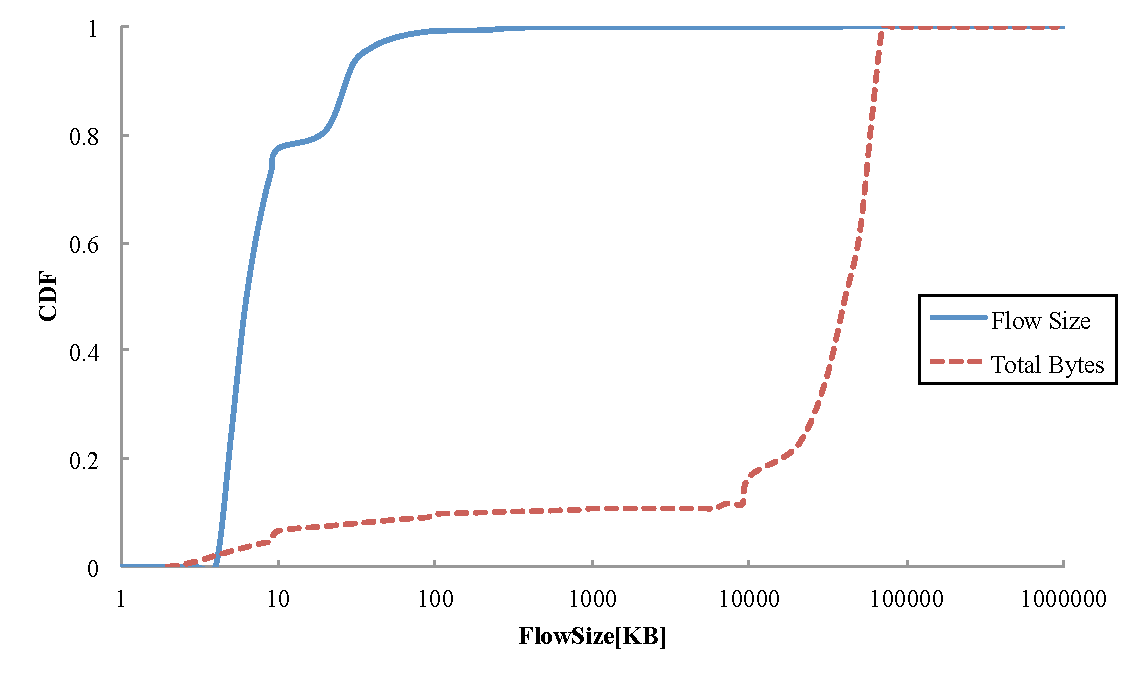
\includegraphics[autoebb, width=250pt]{./img/datamining.pdf}
    \caption{Data mining workload}
    %\ecaption{The control loop in DCTCP}
    \label{fig:datamining}
    \end{center}
\end{figure}

\begin{table}[t]
    \begin{center}
    \caption{The detail of websearch and data mining workload with statistic
    approarch}
    \begin{tabular}{c||c|c}
    \hline
    Workload for & Websearch & Data-mining \\ \hline
    Front-end & \shortstack{Pareto-distribution \\ $a=1.5, \mu=50[KB]$} &
    \shortstack{Pareto-distribution \\ $a=1.5, \mu=10[KB]$} \\ \hline
    Back-end & \shortstack{Pareto-distribution \\ $a=1.2, \mu=10[MB]$} & 
    \shortstack{800[MB]/$n$ bytes \\ from $n$ differrent nodes}
    \end{tabular}
    \label{table:workload}
    \end{center}
\end{table}

Fig.\ref{fig:websearch_FCT_ave}にウェブ検索トラフィックでのショートフロー(0, 100KB]の平均FCTを示す. 
横軸は, バックエンドノードに対する通信負荷の割合$Load$, 縦軸には平均FCTを示す. 
ウェブ検索トラフィックの特徴として, バックエンドへのトラフィックが平均フローサイズ10MBのデータ転送が定期的に生じるということがある. 
これは, 非常に大きなロングフローが継続的に通信するのではなく, 細かく通信が発生することを意味している. 
デッドラインベースの経路切替手法では, たとえSLが混雑していても, デッドライン時間に達するまではLLに切り替わることはできない. 
そのため今回のように, SLでショートフローが頻繁に発生している中で, ロングフローが発生する状況には遅延が生じる. 
一方, リンクコストベースの経路切替手法ではそういった経路の変化に対し, 経路切替のタイミングを変化させて, ショートフローの遅延を最小限に抑えることができる. 
そのため, この結果からわかるように, リンクコストベースの経路切替手法ではFCTが改善できている. 
しかし, Fig.\ref{fig:websearch_FCT_ave}の縦軸の範囲からもわかるように, 基本的にフロントエンドへのフローのサイズが小さいので,
遅延の影響を受ける確率は小さくなり, 大部分のフローが遅延なく通信を完了する. 
そのため提案手法による優位性はあるものの, 改善の度合いは小さい. 

\begin{figure}[t]
    \begin{center}
    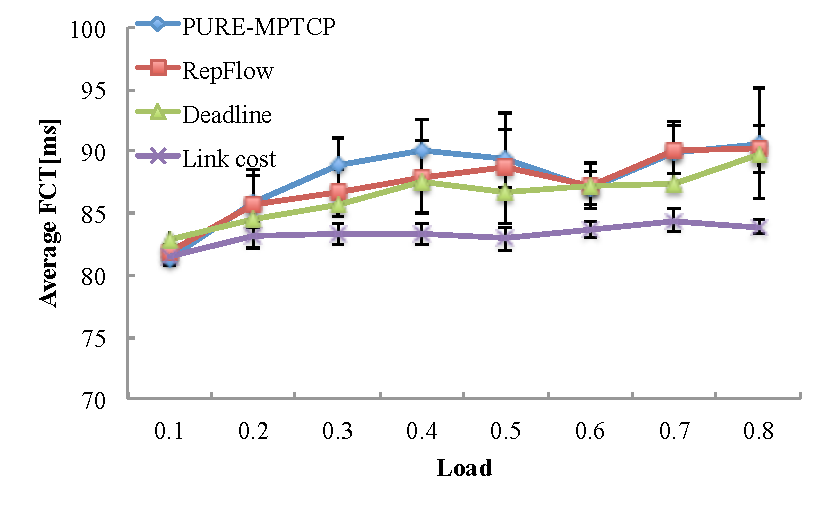
\includegraphics[autoebb, width=250pt]{./img/websearch_avr.pdf}
    \caption{Short flows(0,100KB] average FCT in Websearch workload}
    %\ecaption{The control loop in DCTCP}
    \label{fig:websearch_FCT_ave}
    \end{center}
\end{figure}

次に, Fig.\ref{fig:websearch_FCT_tail}にウェブ検索トラフィックでのショートフロー(0,
100KB]の99パーセンタイルFCTを示す.
横軸はバックエンドノードに対する通信負荷の割合$Load$, 縦軸には99パーセンタイルFCTを示している. 
この結果から提案手法では特に遅延したフローの割合についても, 従来手法より改善することができていることがわかる. 
特に通信負荷を大きくしてった際に, その傾向が顕著に現れる. 
これはPure-MPTCPとRepFlowには, ショートフローとロングフローを公平に扱って通信を行うため, 同一の経路を利用し, Queue
buildupのような性能障害が生じるためである. 
RepFlowは通信負荷が小さい時には, Queue buildupの影響が小さい経路を避けて通信することができるため,
Pure-MPTCPよりも改善することができているが, 通信負荷を大きくしていくとその改善の効果も小さくなっていく. 
一方, 提案手法ではデータセンターレーンモデルによりロングフローとショートフローを区別して通信を制御できるため,
従来手法よりもロングフローの影響を緩和できている. 
しかし, 経路切替の実装上, 通信開始直後にはSLで通信するショートフローに対し, 遅延を生じさせてしまう. 
これにより, デッドラインベースの切替手法では, 通信負荷が大きくなるにつれ, ショートフローへのQueue buildupによる遅延の影響が大きくなる.
それに対し, リンクコストベースの切替手法では, SLに対する影響を抑えることができ, 通信負荷を大きくしても, 遅延が生じるフローの割合を抑えることができる. 


\begin{figure}[t]
    \begin{center}
    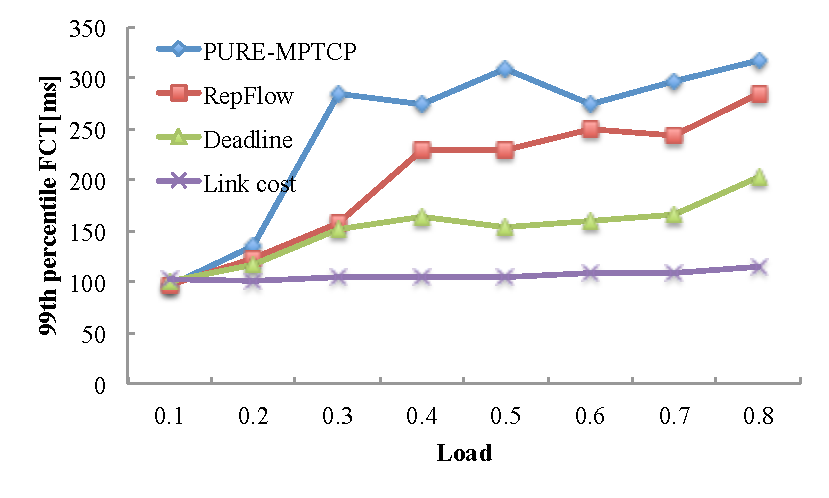
\includegraphics[autoebb, width=250pt]{./img/websearch_tail.pdf}
    \caption{Short flows(0,100KB] $99^{th}$ FCT in Websearch workload}
    %\ecaption{The control loop in DCTCP}
    \label{fig:websearch_FCT_tail}
    \end{center}
\end{figure}

次にFig.\ref{fig:datamining_FCT_ave}にデータマイニングトラフィックでのショートフロー(0, 100KB]の平均FCTを示す. 
横軸はバックエンドノードに対する通信負荷の割合$Load$, 縦軸には平均FCTを示す. 
データマイニングトラフィックトラフィックの特徴として, バックエンドへのトラフィックが非常に大きなデータ転送が継続的に行われる点がある. 
これは, バックエンドに対して通信されるフローの数そのものが少ないことを示しており, 提案手法での通信開始直後のSLに対する影響も小さいということである. 
また, フロントエンドへのトラフィックでは, フローサイズが比較的小さい. 
そのため, ラウンドトリップ回数も少なくなり, 遅延が生じる可能性も小さくなるため,
どの手法においても大部分のフローについては遅延の影響なく通信を完結している. 

\begin{figure}[t]
    \begin{center}
    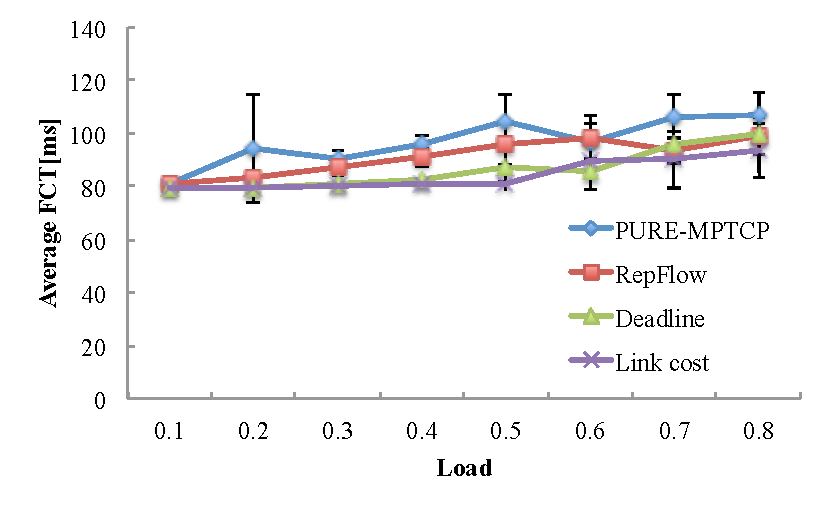
\includegraphics[autoebb, width=250pt]{./img/mining_avr.pdf}
    \caption{Short flows(0,100KB] average FCT in Datamining workload}
    %\ecaption{The control loop in DCTCP}
    \label{fig:datamining_FCT_ave}
    \end{center}
\end{figure}

最後に, 
Fig.\ref{fig:datamining_FCT_tails}にデータマイ二ングトラフィックでのショートフローの99パーセンタイルFCTを示す.
横軸はバックエンドノードに対する通信負荷の割合$Load$, 縦軸には99パーセンタイルFCTを示している. 
この結果から, 二つの提案手法では従来手法と比較し, 大きな遅延が生じたフローの割合について改善できていることがわかる. 
データマイニングトラフィックのバックエンドへのフローに対し, フロー自体は極めて大きなものであるものの,
その数は小さいために通信開始時のSLへの影響が深刻ではなくなっている. 
したがって, データマイニングトラフィックのような粗い粒度でロングフローが発生するようなトラフィックに対しては,
データセンターレーンモデルによるフローの区別によって大きな改善は見られるものの,
経路状況に合わせたリンクコストベースの経路切替手法による改善を期待できる部分が小さいので, 両者における改善の差は小さい. 
\begin{figure}[t]
    \begin{center}
    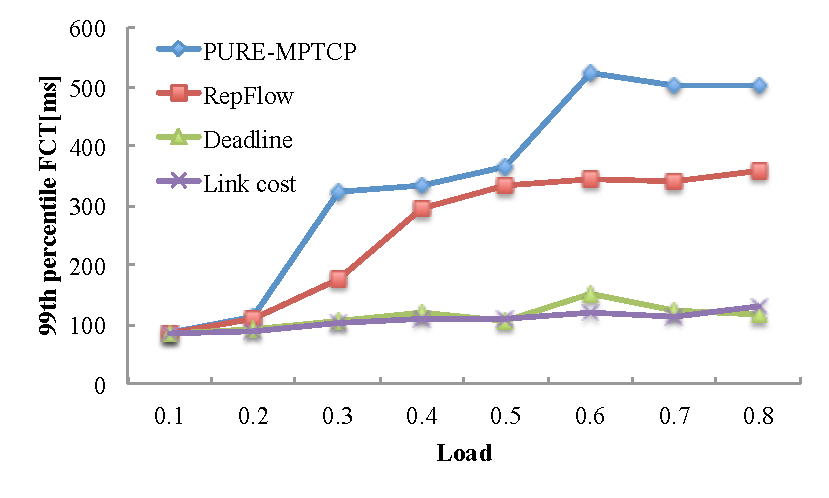
\includegraphics[autoebb, width=250pt]{./img/mining_tail.pdf}
    \caption{Short flows(0,100KB] $99^{th}$ FCT in Datamining workload}
    %\ecaption{The control loop in DCTCP}
    \label{fig:datamining_FCT_tails}
    \end{center}
\end{figure}


\section{まとめ}
データセンターレーンモデルでは,
サイズが小さく素早く通信を完了したいショートフローとサイズが大きく可能な限りたくさんのでデータを転送したいロングフローとを区別し,
個別に通信を行うよう制御することにより, Queue buildupのようにロングフローがショートフロー通信を劣化させる問題を解消している. 
また, エンドノードOSへのアプローチを取る以上, 通信開始当初のフローが区別できない状態において, ロングフローがSLに対し,
キューイング遅延を引き起こす可能性がある.
この問題に対し, リンクコストベースの経路切替手法では, 単純なデッドラーンベースの切替手法とは異なり, 経路の環境に合わせた制御を実現しており,
通信開始当初のSLへの影響を抑制することができる. 

以上の提案手法は, キューイング遅延が直接生じているスイッチに対する変更が不要で, エンドノードのOSに対する変更のみで実現ができる. 
同様の指針で設計された手法としてRepFlowがあり, キューイング遅延が大きい経路を避けて通信することができ,
既存のMPTCPよりも通信性能改善することが可能である. 
しかし, それぞれの要求の異なるショートフローとロングフローが混在し, それらを公平に扱い通信するために, 通信負荷が大きくなった際に通信性能が劣化する. 
これに比べ, 提案手法では指向を区別し, それぞれのフローが干渉しないような制御を行うことで, 通信性能劣化の問題を解決することができた. 
また, エンドノードOSに対する変更のみでの改善, また実際のデータセンターでのトラフィックを想定した評価によって,
提案手法によるショートフローの改善の実用性についても評価することができた. 

